%%%%%%%%%%%%%%%%%%%%%%%%%%%%%%%%%%%%%%%%%%%%%%%
%
% Template per Elaborato di Laurea
% DISI - Dipartimento di Ingegneria e Scienza dell’Informazione
%
% update 2015-09-10
%
% Per la generazione corretta del 
% pdflatex nome_file.tex
% bibtex nome_file.aux
% pdflatex nome_file.tex
% pdflatex nome_file.tex
%
%%%%%%%%%%%%%%%%%%%%%%%%%%%%%%%%%%%%%%%%%%%%%%%

% formato FRONTE RETRO
\documentclass[epsfig,a4paper,11pt,titlepage,twoside,openany]{book}
\usepackage{epsfig}
\usepackage{plain}
\usepackage{setspace}
\usepackage[paperheight=29.7cm,paperwidth=21cm,outer=1.5cm,inner=2.5cm,top=2cm,bottom=2cm]{geometry} % per definizione layout
\usepackage{titlesec} % per formato custom dei titoli dei capitoli

%to have H
\usepackage{float}

%%%%%%%%%%%%%%
% supporto lettere accentate
%
%\usepackage[latin1]{inputenc} % per Windows;
\usepackage[utf8x]{inputenc} % per Linux (richiede il pacchetto unicode);
%\usepackage[applemac]{inputenc} % per Mac.

\singlespacing

\usepackage[italian]{babel}

\begin{document}

  % nessuna numerazione
  \pagenumbering{gobble} 
  \pagestyle{plain}

\thispagestyle{empty}

\begin{center}
  \begin{figure}[h!]
    \centerline{
\psfig{file=marchio_unitrento_colore_it_202002.eps,width=0.6\textwidth}}
  \end{figure}

  \vspace{2 cm} 

  \LARGE{Dipartimento di Ingegneria e Scienza dell’Informazione\\}

  \vspace{1 cm} 
  \Large{Corso di Laurea in\\
    Informatica
  }

  \vspace{2 cm} 
  \Large\textsc{Elaborato finale\\} 
  \vspace{1 cm} 
  \Huge\textsc{DISI Challenge\\}
  \Large{\it{Sviluppo e progettazione di un estensione per DISI Industry}}


  \vspace{2 cm} 
  \begin{tabular*}{\textwidth}{ c @{\extracolsep{\fill}} c }
  \Large{Supervisore} & \Large{Laureando}\\
  \Large{Prof. Paolo Giorgini  }& \Large{Stefano Dal Mas}\\
  \Large{Prof. Alessandro Tomasi }& \\ 
  \end{tabular*}

  \vspace{2 cm} 

  \Large{Anno accademico 2022/2023}
  
\end{center}



  \clearpage
 
%%%%%%%%%%%%%%%%%%%%%%%%%%%%%%%%%%%%%%%%%%%%%%%%%%%%%%%%%%%%%%%%%%%%%%%%%%
%%%%%%%%%%%%%%%%%%%%%%%%%%%%%%%%%%%%%%%%%%%%%%%%%%%%%%%%%%%%%%%%%%%%%%%%%%
%% Nota
%%%%%%%%%%%%%%%%%%%%%%%%%%%%%%%%%%%%%%%%%%%%%%%%%%%%%%%%%%%%%%%%%%%%%%%%%%
%% Sezione Ringraziamenti opzionale
%%%%%%%%%%%%%%%%%%%%%%%%%%%%%%%%%%%%%%%%%%%%%%%%%%%%%%%%%%%%%%%%%%%%%%%%%%
%%%%%%%%%%%%%%%%%%%%%%%%%%%%%%%%%%%%%%%%%%%%%%%%%%%%%%%%%%%%%%%%%%%%%%%%%%
  \thispagestyle{empty}

\begin{center}
  {\bf \Huge Ringraziamenti}
\end{center}

\vspace{4cm}


\emph{
    OpenAI
}

  \clearpage
  \pagestyle{plain} % nessuna intestazione e pie pagina con numero al centro

  
  % inizio numerazione pagine in numeri arabi
  \mainmatter

%%%%%%%%%%%%%%%%%%%%%%%%%%%%%%%%%%%%%%%%%%%%%%%%%%%%%%%%%%%%%%%%%%%%%%%%%%
%%%%%%%%%%%%%%%%%%%%%%%%%%%%%%%%%%%%%%%%%%%%%%%%%%%%%%%%%%%%%%%%%%%%%%%%%%
%% Nota
%%%%%%%%%%%%%%%%%%%%%%%%%%%%%%%%%%%%%%%%%%%%%%%%%%%%%%%%%%%%%%%%%%%%%%%%%%
%% Si ricorda che il numero massimo di facciate e' 30.
%% Nel conteggio delle facciate sono incluse 
%%   indice
%%   sommario
%%   capitoli
%% Dal conteggio delle facciate sono escluse
%%   frontespizio
%%   ringraziamenti
%%   allegati    
%%%%%%%%%%%%%%%%%%%%%%%%%%%%%%%%%%%%%%%%%%%%%%%%%%%%%%%%%%%%%%%%%%%%%%%%%%
%%%%%%%%%%%%%%%%%%%%%%%%%%%%%%%%%%%%%%%%%%%%%%%%%%%%%%%%%%%%%%%%%%%%%%%%%%

    % indice
    \tableofcontents
    \clearpage
    
    
          
    % gruppo per definizone di successione capitoli senza interruzione di pagina
    \begingroup
      % nessuna interruzione di pagina tra capitoli
      % ridefinizione dei comandi di clear page
      \renewcommand{\cleardoublepage}{} 
      \renewcommand{\clearpage}{} 
      % redefinizione del formato del titolo del capitolo
      % da formato
      %   Capitolo X
      %   Titolo capitolo
      % a formato
      %   X   Titolo capitolo
      
      \titleformat{\chapter}
        {\normalfont\Huge\bfseries}{\thechapter}{1em}{}
        
      \titlespacing*{\chapter}{0pt}{0.59in}{0.02in}
      \titlespacing*{\section}{0pt}{0.20in}{0.02in}
      \titlespacing*{\subsection}{0pt}{0.10in}{0.02in}
      
      % sommario
      \chapter*{Sommario} % senza numerazione
\label{sommario}

\addcontentsline{toc}{chapter}{Sommario} % da aggiungere comunque all'indice





Nel corso di questa tesi viene affrontato lo sviluppo dell'applicativo DISI Challenge, una soluzione che permette alle compagnie di formalizzare e pubblicare in un portale delle Challenge, ossia delle sfide che possono variare per estensione temporale, ad esempio delle Capture The Flag o degli Hackaton in generale di durata 1-2 giorni, piuttosto che delle sfide a lunga durata dove viene richiesto di effettuare il design ed eventualmente l'implementazione di un progetto che risolva una task specifica fornita. Il vantaggio dell'esistenza di un tale applicativo è il ridurre al minimo l'affaticamento dovuto alla ricerca di questa tipologia di opportunità da parte degli studenti, permettendo loro di avere un unica soluzione che possa in modo semplice ed intuitivo raccogliere tali sfide, formando un gruppo per parteciparvi, mentre per le aziende è più facile avere una maggiore pubblicità per le iniziative proposte, con quindi una maggiore possibilità di trovare un eventuale soluzione ad un problema posto o trovare in maniera più efficiente ed efficace dei nuovi talenti da introdurre eventualmente nel contesto lavorativo.

Al momento di una pubblicazione di una Challenge da parte dell'azienda all'interno dell'applicativo, il moderatore, ossia una figura che gestisce uno o più laboratori all'interno dell'università, approva o rifiuta una Challenge con lo scopo di mantenere alta la qualità delle proposte per gli studenti. All'accettazione di una nuova Challenge da parte del moderatore, agli studenti viene reso disponibile l'iscrizione, creando un gruppo o entrando a far parte di uno già esistente, chiedendo la partecipazione ad un Tutor, ossia una figura all'interno del DISI incaricata della supervisione di un gruppo formato per partecipare ad una Challenge. Una volta che il Tutor ha accettato di entrare a far parte del gruppo, l'azienda può visualizzare il dettaglio dei gruppi iscritti e muniti di tutor ed hanno la possibilità di decidere se il suddetto possa partecipare o meno alla Challenge. Tale processo è stato disegnato per permettere di avere un controllo di qualità sia da parte dell'azienda, che da parte dei singoli studenti, così da evitare spiacevoli inconvenienti durante l'arco della Challenge.


In primo luogo è stata presentata l'idea iniziale al Dott. Giorgini, nata dalla mia partecipazione a delle Challenge promosse all'interno dell'università di Trento, come ad esempio il progetto Samsung Innovation Camp, promosso da Samsung, e dal mio desiderio di permettere agli studenti di poter parteciparvi in modo semplice ed intuitivo per permettere di massimizzare le partecipazioni a queste iniziative.

Dopo aver ricevuto un riscontro positivo per l'idea, la prima parte del progetto è stata investita nell'analizzare se esistessero già delle realtà nelle quali tale opportunità esisteva, ed è lì che ho incontrato l'applicativo DISI Industry, WebApp volta al permettere alle aziende di pubblicare offerte di lavoro o di tirocinio, così da ottenere il miglior candidato possibile per il ruolo da ricoprire, mentre allo studente è disponibile una piattaforma nella quale può trovare delle offerte che siano più in linea possibile con i suoi desideri e le sue competenze, il tutto mediante un unico applicativo. Mi è parsa dunque un'ottima idea implementare la mia soluzione all'interno di quest'ultimo proprio per la natura simile tra la mia ideologia e quella di DISI Industry, cosìda ampliare l'offerta di quest'ultima, ponendo maggiore enfasi al collegamento tra il mondo accademico e quello dell'industria.

Successivamente si è passati ad un'analisi delle tecnologie utilizzate da DISI Industry, cercando di comprendere appieno il funzionamento dei framework e dei sistemi adottati, per permettere di sviluppare una soluzione che fosse il più coerente e compatibile con la codebase già esistente, in modo da permettere all'utente finale di fruire dei due applicativi senza interruzione di continuità, in modo semplice e fluido, mantenendo dunque lo stile architetturale e grafico per non stravolgere l'esperienza dell'utente finale.


Dopo aver effettuato tale analisi, si è passati ad una definizione più formale di che cosa fosse necessario per formalizzare e comporre una Challenge, oltre che degli attori del sistema e dei correlati requisiti funzionali, ossia di chi può fare cosa all'interno della WebApp, concludendo con lo studio del processo sopracitato per la creazione di una Challenge e la conseguente partecipazione degli studenti ad essa utilizzando DISI Challenge.

Un'ulteriore fase, dipendente dalla definizione degli attori e dallo studio delle tecnologie utilizzate, è stata l'analisi di contesto, necessaria per comprendere appieno come il modulo si interfacciasse agli strumenti già esistenti in DISI Industry ed agli attori definiti in precedenza, così da poter comprendere appieno come il modulo si inserisse all'interno del sistema già esistente, in modo da poterlo integrare senza stravolgere l'esperienza dell'utente finale.

Ulteriore fase di necessaria importanza è stata la modellazione del Back-End per permettere la realizzazione di tali funzionalità e lo sviluppo del Front-End per ottenere un'esperienza gradevole e coerente al portale DISI Industry.

Per quanto concerne il risultato finale, l'applicazione ha percepito un'ingrandimento dell'idea iniziale con l'inserimento di un sistema di Feedback. Esso permette in primo luogo di fornire dei riscontri da parte delle aziende, quindi di figure esperte nel settore, in base alla performance agli studenti. In secondo luogo a questi ultimi viene permesso di fornire delle risposte alle aziende, così da permettere a queste ultime di comprendere e migliorare le future Challenges che verranno proposte, ma anche per permettere ad altri studenti di avere un metro di paragone fornito dai loro colleghi durante la ricerca di nuove Challenges nel portale.

DISI Challenge è dunque risultato un progetto, che si è risolto nello sviluppo di un modulo per la WebApp DISI Industry, che rispecchia i requisiti definiti inizialmente. Tra i possibili sviluppi futuri vi sono l'ottimizzazione e la rifinitura di alcune query poste al back-end, oltre ad una rifinitura all'interfaccia front-end, la quale è stata sviluppata per permettere all'utente di utilizzare l'applicativo senza però porre troppa attenzione alle rifiniture. Tale scelta è stata adottata per permettere di proporre alla fine del lavoro un'applicazione leggermente meno rifinita ma completa di tutte le funzionalità richieste, piuttosto che rimuovere alcune di esse per prediligere la qualità dell'interfaccia grafica, che resta comunque elevata data la struttura iniziale di DISI Industry.

Un altro sviluppo futuro possibile è l'implementazione di una Chat all'interno del modulo, che permetta alle aziende ed ai gruppi formati in occasioni di varie Challenges, di poter comunicare all'interno del portale senza dover occorrere a soluzioni e metodologie esterne, così da ridurre ulteriormente il carico da parte degli utenti finali e migliorarne l'esperienza.

%%%%%%%%%%%%%%%%%%%%%%%%%%%%%%%%%%%%%%%%%%%%%%%%%%%%%%%%%%%%%%%%%%%%%%%%%%
%%%%%%%%%%%%%%%%%%%%%%%%%%%%%%%%%%%%%%%%%%%%%%%%%%%%%%%%%%%%%%%%%%%%%%%%%%
%% Nota
%%%%%%%%%%%%%%%%%%%%%%%%%%%%%%%%%%%%%%%%%%%%%%%%%%%%%%%%%%%%%%%%%%%%%%%%%%
%% Sommario e' un breve riassunto del lavoro svolto dove si descrive 
%% l’obiettivo, l’oggetto della tesi, le metodologie e 
%% le tecniche usate, i dati elaborati e la spiegazione delle conclusioni 
%% alle quali siete arrivati.
%% Il sommario dell’elaborato consiste al massimo di 3 pagine e deve contenere le seguenti informazioni: 
%%   contesto e motivazioni
%%   breve riassunto del problema affrontato
%%   tecniche utilizzate e/o sviluppate
%%   risultati raggiunti, sottolineando il contributo personale del laureando/a
%%%%%%%%%%%%%%%%%%%%%%%%%%%%%%%%%%%%%%%%%%%%%%%%%%%%%%%%%%%%%%%%%%%%%%%%%%
%%%%%%%%%%%%%%%%%%%%%%%%%%%%%%%%%%%%%%%%%%%%%%%%%%%%%%%%%%%%%%%%%%%%%%%%%%      
      
      %%%%%%%%%%%%%%%%%%%%%%%%%%%%%%%%
      % lista dei capitoli
      %
      % \input oppure \include
      %
      \chapter{Introduzione ed obbiettivi }
\label{cha:intro}
In questo primo capitolo introduttivo vengono spiegati i motivi che hanno portato la realizzazione del progetto "DISI Challenge" ed una presentazione di "DISI Industry", la piattaforma per la quale è stato integrato il modulo è stato sviluppato. Vengono inoltre presentati gli obbiettivi che si vogliono raggiungere con la realizzazione del progetto.
Iniziando da questi ultimi, il progetto ha come obbiettivo la realizzazione di una WebApp sottoforma di modulo da poter aggiungere alla piattaforma DISI Industry, ossia una piattaforma già esistente che permette la mediazione tra il mondo accademico ed il mondo del lavoro ed industria in modo semplice ed efficace. Vi devono essere molteplici tipologie di attori, tra i quali studenti, manager di compagnie, moderatori e tutor universitari, ognuno con dei privilegi differenti all'interno della piattaforma. 


L'applicativo DISI Challenge deve permettere alle aziende, enti esterni all'università, di poter formalizzare e proporre delle "Challenge". Esse vengono definite come gare a lungo termine ove viene richiesto ai gruppi partecipanti di effettuare sia la fase di progettazione che eventualmente la fase implementativa di una soluzione rispetto ad un problema definito, oppure può essere proposta sottoforma di hackaton, ossia una competizione volte alla risoluzione di un problema in un lasso di tempo limitato mettendo in palio una serie di premi per i team vincitori. In questa relazione tra company manager(creatori di Challenges) e studenti(partecipanti alle varie Challenges), vi devono essere delle figure intermedie quali i Moderatori, incaricati di verificare se la Challenge proposta dal Company manager sia consona e possa essere proposta agli studenti, ed i Tutor, figure incaricate della supervisione degli studenti alla formazione di un gruppo per partecipare alla Challenge designata.

Un esempio di Challenge che rientrano in questa categoria sono le Reply Challenge, hackaton nelle quali ai gruppi viene richiesto di risolvere dei problemi di algoritmica e di programmazione, oppure le Capture The Flag, hackaton nell'ambito della Cyber Security nel quale dei team concorrono contro l'organizzatore, oppure tra di loro, cercando di attaccare o difendere un sistema non sicuro.

Questo progetto nasce dalla mia partecipazione al Samsung Innovation Camp, un evento proposto da Samsung in collaborazione con Randstad, nel quale veniva richiesto agli studenti di risolvere una problematica proposta dall'azienda, differenziandola sulla base dell'ateneo scelto, proponendo soluzioni che sfruttassero le nuove tecnologie quali Internet of Things, Intelligenza Artificiale e tutte le nuove tecnologie correlate. La problematica proposta all'ateneo di Trento era inerente alla valorizzazione del patrimonio naturalistico, artistico e culturale mediante l'innovazione digitale, con l'obbiettivo di sostenere il settore della Cultura e del Turismo.

La partecipazione a tale progetto mi ha permesso di conoscere nuove tecnologie, meccaniche aziendali e di lavorare in un team di sviluppo, permettendomi di migliorare le mie capacità di problem solving, di lavoro in team e di gestione del tempo, facendomi inoltre realizzare quanto sia importante avere una piattaforma nella quale gli studenti possano in modo semplice e veloce trovare tutte le informazioni necessarie per partecipare alle Challenge proposte dalle aziende.

Ho dunque deciso di implementare questa WebApp per permettere di ridurre lo spazio tra le aziende e l'università, fornendo dunque un portale nel quale questo tipo di interazioni, volte ad un applicazione pratica di quanto imparato durante il percorso universitario, siano facilmente accessibili agli studenti.



\section{DISI Industry}
\label{sec:context}
Durante la fase embrionale del progetto, ancora prima di iniziare a definire i requisiti, ho effettuato delle ricerche per vedere se esistessero già soluzioni simili o comunque compatibili con la mia idea, ed ho trovato il progetto DISI Industry.


La scelta dell'integrazione di questo modulo all'interno di una WebApp già esistente è sorta dal fatto che DISI industry nasce già con l'idea di connettere gli studenti con l'industria, in quanto i primi possono cercare delle offerte di lavoro comparabili con le loro competenze apprese durante gli studi, mentre le compagnie possono offrire ruoli di lavoro per trovare il personale più adatto alle loro richieste. Essa può essere dunque definita come una piattaforma di recruiting online per gli studenti del DISI ed il suo ruolo all'interno dell'ambiente universitario è estremamente importante, in quanto permette di ridurre il divario tra il mondo accademico e quello dell'industria. \cite{industry}

Mi è dunque venuta naturale l'idea di implementare il modulo all'interno della WebApp per l'affinità intrinseca tra la mia ideologia e quella proposta dalla piattaforma già esistente, così da permettere agli studenti non solo di poter cercare potenziali offerte di tirocinio o di lavoro, ma anche di poter partecipare a delle Challenge proposte dalle aziende, così da poter mettere in pratica le proprie conoscenze e competenze apprese durante il percorso universitario, di poterle migliorare, oltre che di poter vincere dei premi ed arricchire il proprio Curriculum Vitae, il tutto mediante la stessa piattaforma per ridurre al minimo la fatica dovuta alla navigazione di molteplici pagine web e portali differenti.




      \chapter{Tecnologie utilizzate}
\label{cha:tecnologie_utilizzate}


In questo capitolo vengono presentate le tecnologie utilizzate e le motivazioni dietro tali scelte. In particolare, vengono presentate le tecnologie utilizzate per la realizzazione del back-end, del front-end e del database.

\section{Django}
Il framework utilizzato è Django, esso è stato scelto per la sua semplicità di utilizzo e per la sua flessibilità. Django è un framework open-source di alto-livello per lo sviluppo di applicazioni web scritto in Python. Esso è basato sul pattern architetturale Model-View-Template (MVT) e permette di sviluppare applicazioni web in modo rapido e pulito, fornendo un'interfaccia di amministrazione per la gestione dei dat, così da non dover implementare un admin zone mediante un altro linguaggio, ma mantenendo unificata la codebase. 

Un altro vantaggio risiede nella scalabilità del framework, il quale permette la creazione di moduli che possono essere inseriti o rimossi con l'aggiunta di poche righe di codice all'interno di un file apposito. 

\subsection{Architettura MVT}
Il vantaggio dell'utilizzo di un framework basato su architettura MVT permette ad ogni livello, ossia Model, View e Template, di lavorare indipendentemente, il che permette una maggiore indipendenza tra le parti. Esso è conveniente nel caso si decida di scalare l'applicativo web, in quanto permette di aggiungere nuove funzionalità senza dover modificare il codice già esistente. Inoltre, un'architettura MVT permette di rendere più veloce e più seplice la trasmissione di dati via internet.


Vengono presentati in dettaglio le componenti dell'architettura MVT:
\begin{itemize}
    \item Model : questo componente aiuta la gestione del database ed esso è un livello di accesso dati che contiene i campi ed il comportamento dei dati che stanno venendo gestiti. Esso utilizza un pattern ORM (Object-Relational Mapping) che mappa i campi del database con gli attributi della classe Python. Questo permette di utilizzare un linguaggio di programmazione orientato agli oggetti come Python per la gestione dei dati, permette un livello di astrazione tale da non rendere obbligatoria la stesura di query in linguaggio SQL, inoltre permette una maggiore semplicità durante la manutenzione del codice dovuta al fatto che solamente un linguaggio viene utilizzato. Mediante ORM è anche possibile cambiare database in modo efficace ed efficiente, in quanto non è necessario modificare il codice già esistente. 
        I modelli aiutano  ad effettuare le operazioni CRUD (Create, Read, Update, Delete) sul database in modo semplice e veloce. Inoltre, Django permette di definire delle relazioni tra i modelli, in modo da poter accedere ai dati in maniera semplice e veloce, oltre alla definizione di ciò che viene definita Business Logic del programma (es. validazione dei dati, ecc.). \cite{django_models}
\item View : Esso può essere visto come l'organoesecutivo della Business Logic, in quanto permette di interagire con i modelli definiti dal modulo Model e  gestisce la renderizzazione in template. La view ottiene i dati dal Model, dopodichè può modificare i suddetti ed eventualmente renderizzarli in un template. Esso accetta richeste HTTP(HyperText Transfer Protocol), applica la business logic e fornisce risposte HTTP al client. \cite{django_views}
    \item Template : Questo modulo è il livello più vicino all'utente, in quanto è un livello di presentazione che gestisce completamente l'interfaccia dell'utente. Essi sono file con codice HTML(HyperText Markup Language) che vengono utilizzati per renderizzare dati ed essi possono contenere dati statici o dinamici. Nel caso di Django viene utilizzato un lingaggio speciale chiamato Django Template, il quale permette la definizione di variabili, cicli, condizioni, ecc. oltre ai comandi classici di HTML. Inoltre, permette di definire un template base, il quale può essere esteso da altri template. \cite{django_template}
\end{itemize}


\subsection{Sicurezza}

Un altro vantaggio del framework Django è la sicurezza, in quanto nativamente supporta dei controlli che possono essere facilmente inclusi sfruttando il livello d'astrazione fornito da un framework. \cite{django_security}

Oltre ai controlli sull'autenticazione, autorizzazione e gestione delle sessioni, tale framework permette di evitare attacchi tra i quali:
\begin{itemize}
    \item SQL Injection : Attacco volto all'inserimento di codice SQL in input non controllati, in modo da poter accedere ai dati del database. Django permette di evitare tale attacco in quanto permette di utilizzare un linguaggio di programmazione orientato agli oggetti come Python per la gestione dei dati, applicando ciò che viene definito \textit{input sanitizing}, il quale permette di evitare l'inserimento di codice SQL in input non controllati.
    \item Cross Site Scripting(XSS) : Tale attacco permette all'utente di inserire codice HTML e JavaScript malevolo che verrà poi visualizzato dagli altri utenti dell'applicazione mediante la pressione di un link o bottone. Tale problema viene risolto mediante input sanitizing e l'escape automatico di caratteri non sicuri.
    \item Cross Site Request Forgery(CSRF): L'attacco CSRF sfrutta il fatto che molte applicazioni web autenticano gli utenti utilizzando sessioni o token di autenticazione, ma non validano in modo appropriato la fonte delle richieste che vengono inviate. In un attacco CSRF, un malintenzionato crea una pagina web malevola o un messaggio e lo fa visualizzare all'utente target mentre è autenticato in un'altra applicazione web.

Quando l'utente visualizza questa pagina o questo messaggio, il codice maligno presente al suo interno genera una richiesta HTTP verso l'applicazione web bersaglio, sfruttando la sessione o il token di autenticazione dell'utente. Poiché l'applicazione web bersaglio considera la richiesta legittima, esegue l'azione richiesta, che potrebbe essere, ad esempio, un trasferimento di fondi, una modifica delle impostazioni dell'account o l'invio di un messaggio. Django permette di evitare tale attacco mediante l'utilizzo di un token di sicurezza.

    \item Clickjacking : Attacco che mira ad ingannare l'utente mediante il click di zone nascoste o trasparenti. Django permette di evitare tale attacco mediante l'utilizzo di un middleware che permette di inserire un'intestazione HTTP.

\end{itemize}


\clearpage

      \chapter{Analisi di Contesto e definizione di Challenge}

In questo capitolo viene introdotta una definzione formalizzata di Challenge, successivamente alla quale viene introdotta un'analisi di contesto, necessaria per la definizione di attori e come essi interagiscono tra loro.

\section{Challenge}
Viene definita \textbf{Challenge} una sfida proposta dall'azienda esterna all'università ed è composta da:
\begin{itemize}
    \item Nome della Challenge.
    \item Laboratorio nel quale si svolgerà.
    \item Descrizione accurata del problema da risolvere.
    \item Data di inizio. 
    \item Data di fine.
    \item Orario.
    \item Autore, ossia il nome dell'azienda.
    \item Descrizione testuale del premio messo in palio dall'azienda per il gruppo vincitore.
    \item Limite temporale per l'iscrizione dei gruppi.
    \item Dimensione di ogni gruppo. 
    \item Numero massimo di gruppi.
\end{itemize}

Ogni azienda può formare più di una Challenge.

Alla conclusione del limite temporale previsto l'azienda che ha creato la Challenge \textbf{deve} selezionare i gruppi che parteciperanno entro un quantitativo di giorni. Gli utenti facenti parte dei gruppi selezionati riceveranno una mail contenente i dati della Challenge con eventuali dettagli aggiuntivi.

Alla conclusione di una Challenge ad ogni studente è richiesto di compilare un form per fornire feedback sull'attività appena svolta per poterlo inviare all'azienda.
L'applicativo non prevede uno strumento di comunicazione tra azienda e studente oltre al form sopracitato.

Vi è una diretta correlazione \textbf{l'area tematica} della challenge proposta dall'azienda ed il \textbf{laboratorio didattico}, in quanto la suddetta può formalizzare una challenge di una specifica area tematica solamente nel laboratorio corrispondente.

Alla creazione della Challenge, essa viene inserita in un Pending state finchè non viene accettata/rifiutata dal moderatore. Dopo tale azione essa entra in uno stato Accettato o Rifiutato in base alla scelta del suddetto.

\section{Attori}
Di seguito vengono riportati gli attori dell'applicativo. Ad ogni attore vengono associati i requisiti funzionali correlati sulla base delle azioni che possono effettuare.

\subsection{Studente}
Uno studente viene definito come una persona iscritta all'Università di Trento e che attualmente ricopre il ruolo di studente del corso di laurea triennale o magistrale, dottorando o ricercatore.

Tale utente può effettuare le seguenti azioni:

\begin{itemize}
    \item Selezionare le aree tematiche al quale è interessato per poter ricevere notifiche alla validazione di nuove Challenge da parte del moderatore.
        \begin{itemize}
            \item Lo studente può decidere di non ricevere email inerenti a nuove Challenge facente parte della sua area tematica.
        \end{itemize}
    \item Visualizzare la lista delle Challenges facenti parte dell'area di interesse selezionata.
    \item Visualizzare informazioni inerenti alla Challenge selezionata.
    \item Iscriversi alla Challenge formando o entrando a far parte di un gruppo.
    \item Al termine di una Challenge lo studente può compilare un form per fornire un feedback all'azienda sulla Challenge appena compiuta. 
    \item Al termine di una Challenge lo studente può visualizzare il feedback ricevuto da parte del Company Manager.
\end{itemize}

Uno studente può avere molteplici aree di interesse e può partecipare a più di una Challenge appartenente al suo settore di interesse.

\subsection{Gruppo di Studenti}
Per poter partecipare ad una Challenge gli studenti devono formare un gruppo. Un gruppo è definito da uno o più studenti ed un Tutor. 
Alla formazione di un nuovo gruppo il primo nominativo diviene il capogruppo ed ad esso viene richiesto di:
 \begin{enumerate}
        \item Fornire il nome per il gruppo.
        \item Selezionare il Tutor del gruppo. 
        \item Fornire una presentazione testuale del gruppo. 
\end{enumerate}

Alla formazione di un gruppo esso è in stato di \textbf{Pending}. Esso può cambiare di stato quando:
\begin{itemize}
    \item Il tutor selezionato visualizza il dettaglio del gruppo ed accetta di farne parte. In tal caso lo stato del gruppo diviene \textbf{Tutored}. 
    \item Il tutor selezionato visualizza il dettaglio del gruppo e rifiura di farna parte. In tal caso lo stato del gruppo diviene \textbf{Rejected}. 
    \item Il Company Manager visualizza il dettaglio del gruppo e lo accetta per partecipare alla Challenge. In tal caso lo stato del gruppo diviene \textbf{Accepted}. 
    \item Il Company Manager visualizza il dettaglio del gruppo e lo rifiuta. In tal caso lo stato del gruppo diviene \textbf{Rejected}. 
\end{itemize}

Per partecipare ad una Challenge è richiesto che il gruppo sia in \textbf{Accepted} state.



\subsection{Moderatore}
Tale figura é incaricata di accettare le Challenges che potranno essere effettuate, oltre al modificare i membri dei gruppi. Ogni Laboratorio ha un solo responsabile. Esso viene riferito anche come \textit{responsabile di laboratorio}.

L'utente può effettuare le seguenti azioni:
\begin{itemize}
    \item Visualizzare tutti i laboratori che gestisce. 
    \item Visualizzare tutte le challenge proposte per quel laboratorio.
    \item Accettare o rifiutare le Challenges proposte dall'azienda.
    \item Prenotare il laboratorio nel caso la Challenge venga accettata. Tale azione è esterna all'applicativo.
    \item Gestire gli account delle aziende(creazione, eliminazione, modifica, etc). Tale azione è esterna all'applicativo.
\end{itemize}


\subsection{Company Manager}

Questo utente viene creato all'interno del Sistema in seguito alla formulazione ed approvazione di una richiesta esterna all'applicativo.

Tale utente può effettuare le seguenti azioni:
\begin{itemize}
    \item Creare una Challenge.
    \item Visualizzare tutte le Challenge che ha effettuato.
    \item Modificare Challenge non accettate o rifiutate.
    \item Accedere al dettaglio della Challenge e visualizzare ogni gruppo.
    \item Accettare o rifiutare l'ingresso di un gruppo ad una determinata Challenge. 
    \item Al termine di una Challenge il Company Manager può fornire il feedback mediante un modulo apposito per il lavoro svolto ad ogni gruppo e studente. 
    \item Al termine di una Challenge il Company Manager può Visualizzare il feedback di tutti gli studenti che hanno partecipato alla Challenge e lo hanno fornito.
\end{itemize}

\subsection{Tutor}
Tale figura è un membro del DISI ed è incaricata della supervisione di un gruppo durante una Challenge. Alla creazione di un gruppo per partecipare ad una Challenge \textbf{deve} essere selezionato. 

Esso può svolgere le seguenti attività:
\begin{itemize}
    \item Visualizzare tutti i gruppi che hanno richiesto la sua partecipazione. 
    \item Accettare di entrare a far parte di un gruppo o rifiutarlo. Si ricordi che all'accettazione da parte del tutor il gruppo entra in \textbf{Tutored }state. 
\end{itemize}

\section{Diagramma di Contesto}

Nel seguente elenco è posisbile trovare una descrizione ad alto livello delle relazioni tra le differenti componente esterne al sistema. Bisogna notare che tale rappresentazione viene effettuata a livello logico e non è correlata all'architettura del framework utilizzato.

Il \textbf{Company Manager} è un \textbf{attore} e può svolgere le seguenti azioni: può effettuare il login, gestire le proprie challenge, accettare o rifiutare i gruppi (già in tutored state, ossia gruppi i quali siano già formati ed accettati da un Tutor), oltre a poter compilare e visualizzare i feedback inerenti alle challenge dell'azienda.

Il \textbf{Moderatore} è un \textbf{attore} e può svolgere le seguenti azioni: può visualizzare i laboratori che modera, accedere al loro dettaglio ed accettare o rifiutare le Challenge proposte per il laboratorio.

Lo \textbf{Studente} è un \textbf{attore} e può svolgere le seguenti azioni: può cambiare i propri interessi in modo da vedere solo le challenge che facciano parte della sua area di interesse, può decidere se essere aggiornato o meno sulle nuove Challenge approvate dal moderatore, formare e gestire i gruppi creati appositamente per le Challenge, fornire e visualizzare i feedback relativi alle Challenge effettuate. 

Il \textbf{Tutor} è un \textbf{attore} e può svolgere le seguenti azioni: può visualizzare i gruppi che hanno richiesto la sua partecipazione, accettare o rifiutare di farne parte.

Il \textbf{Sistema di invio mail/notifica} è l'infrastruttura che permette l'invio di email nei seguenti casi ed ai seguenti attori:
\begin{itemize}
    \item Creazione di una nuova Challenge da parte del Company Manager : viene inviata una mail a tutti i moderatori del laboratorio nella quale la Challenge deve essere svolta. 
    \item Accettazione o rifiuto di una Challenge da parte del Moderatore: viene inviata una mail al Company Manager che ha creato la Challenge, oltre che ad una mail a tutti gli studenti che hanno richiesto di essere aggiornati sulle nuove Challenge e i quali interessi siano un super-set della Challenge accettata.
    \item Creazione di un nuovo gruppo da parte di uno studente : viene inviata una mail al Tutor selezionato dal capogruppo.
    \item Accettazione o rifiuto di entrare a far parte di un gruppo da parte del Tutor : viene inviata una mail a tutti i membri del gruppo.
    \item Accettazione o rifiuto di un gruppo da parte del Company Manager : viene inviata una mail a tutti i membri del gruppo.
\end{itemize}

\textbf{Shibboleth} è il modulo che permette di effettuare il login all'interno dell'applicativo. Esso è un software open source che permette l'autenticazione federata e single sign-on.

Il \textbf{Database} è il corrispondente di ciò che è stato definito come componente Model all'interno dell'architettura di Django. Esso gestisce le transazioni con il Database ed è l'unico modulo in grado di accedere ai dati. Esso permette la traduzione di query da linguaggio python al linguaggio della base di dati selezionata. 

Di seguito viene riportato il diagramma di contesto dell'applicativo.


\begin{figure}
    \centering
    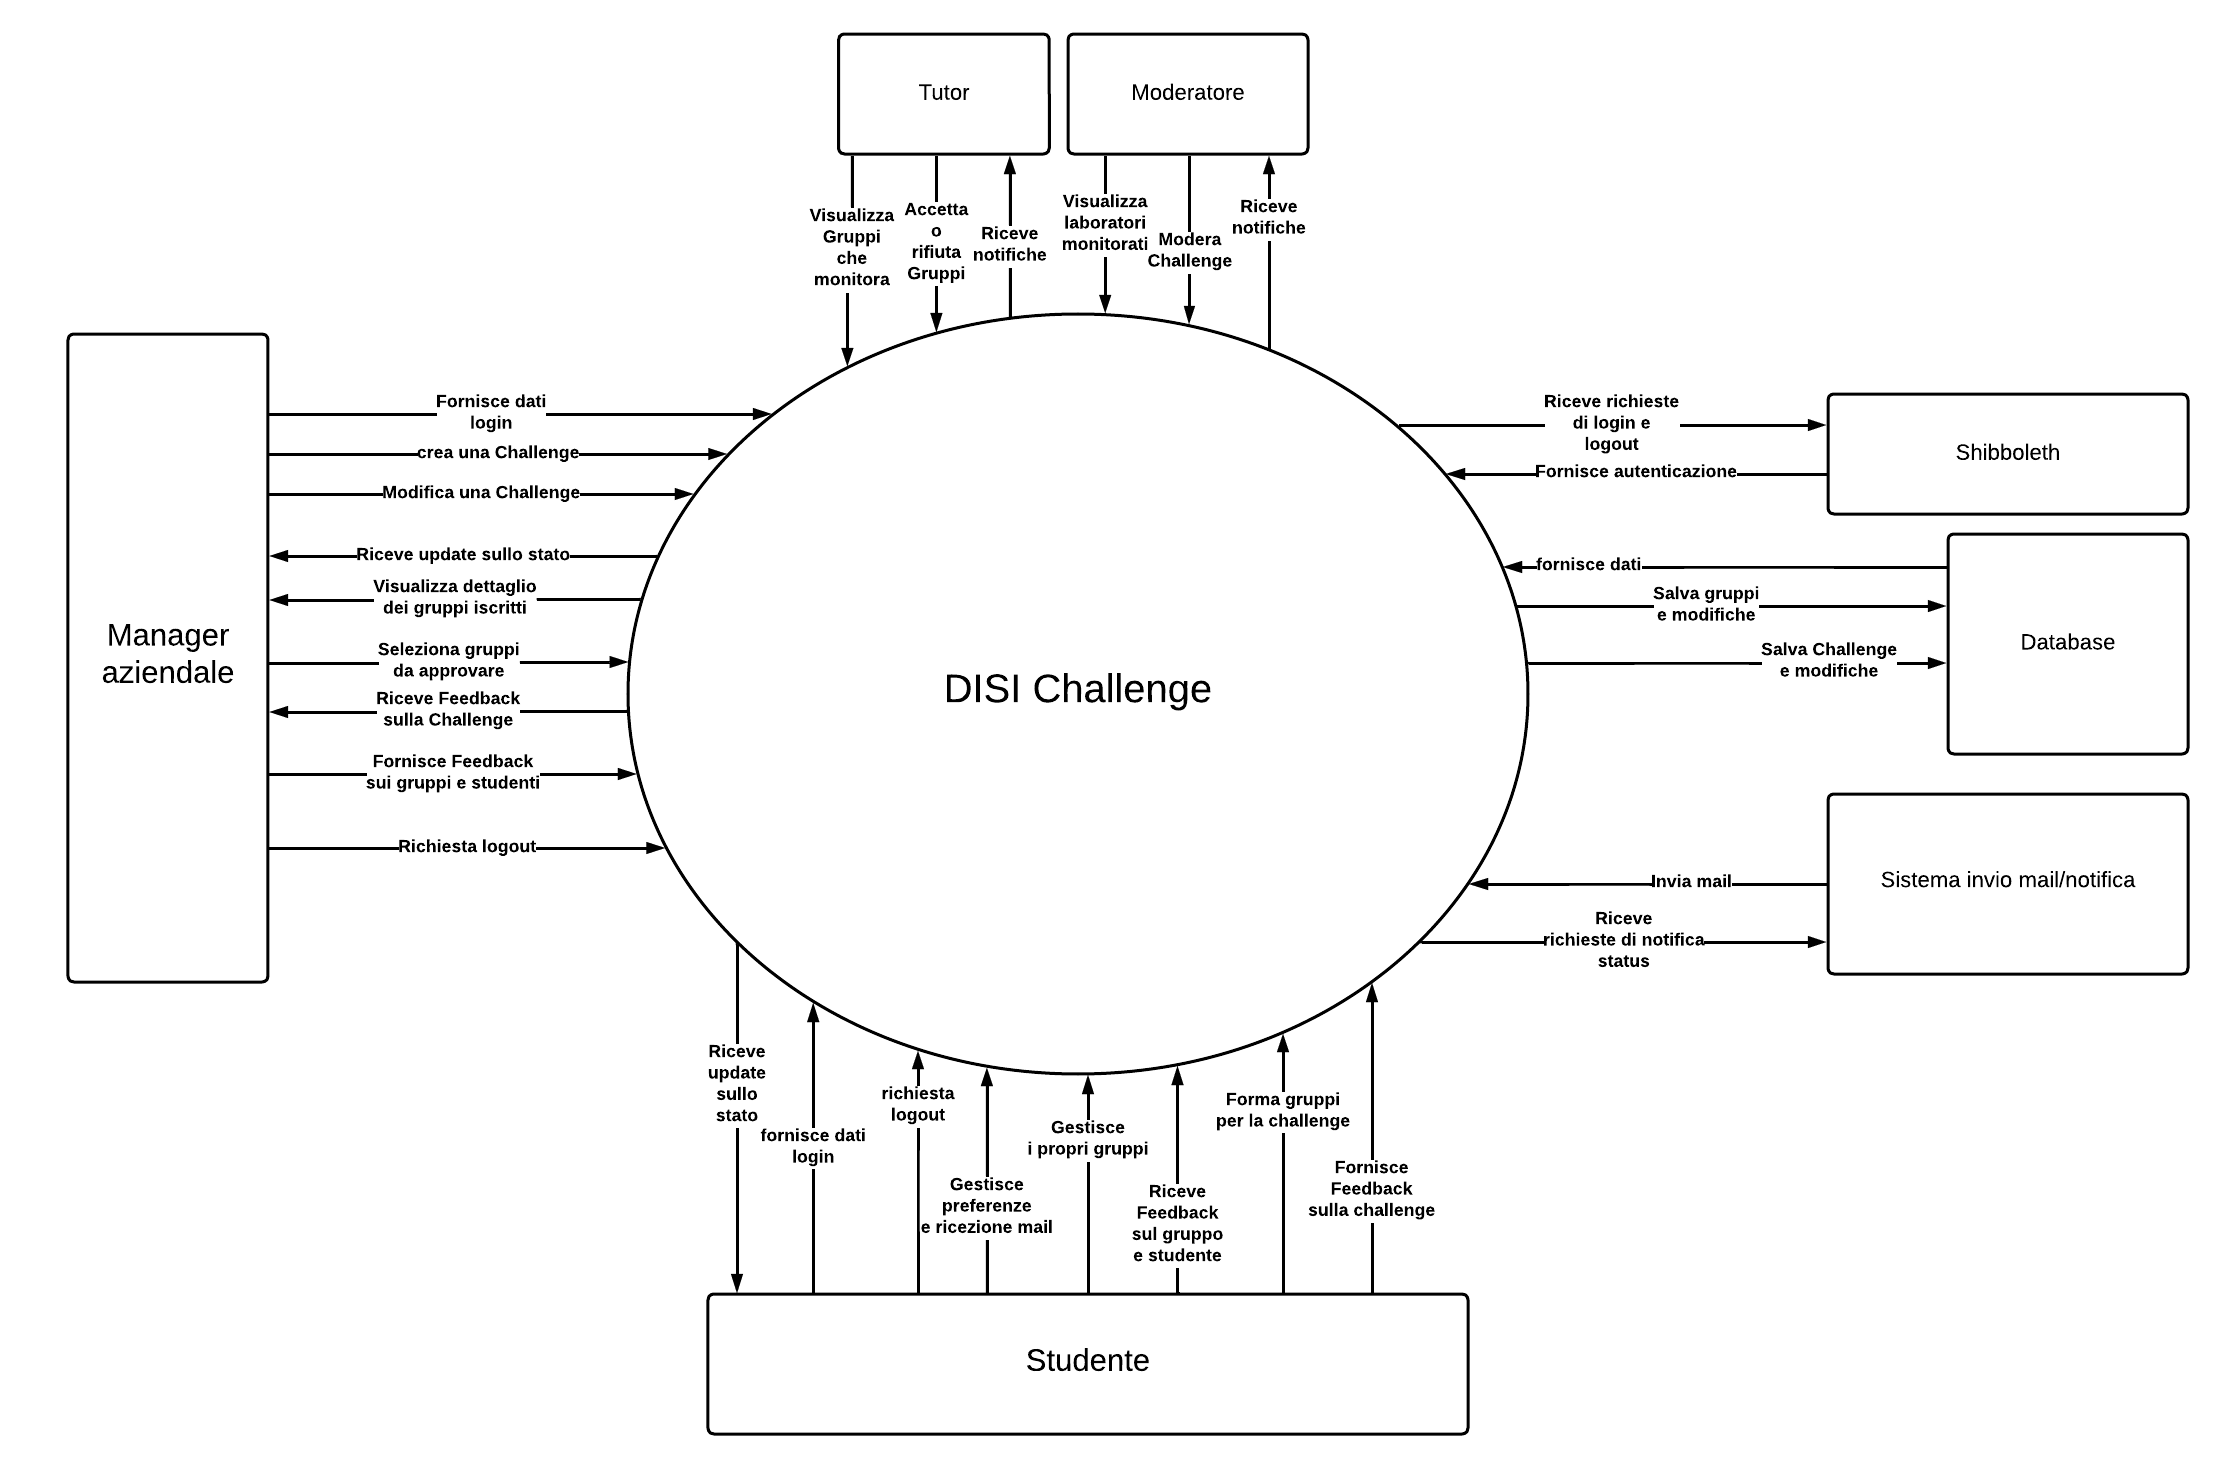
\includegraphics[scale=0.46]{images/diagrama_di_contesto.png}
    \label{fig:diagrama_di_contesto}
    \caption{Diagramma di contesto}
\end{figure}

\section{Processo di creazione e partecipazione ad una Challenge}

Data la complessità del processo, viene di seguito utilizzato un diagramma Business Process Model Notation (BPMN) per descrivere il processo di creazione e partecipazione ad una Challenge. 

\begin{figure}[ht]
    \centering
        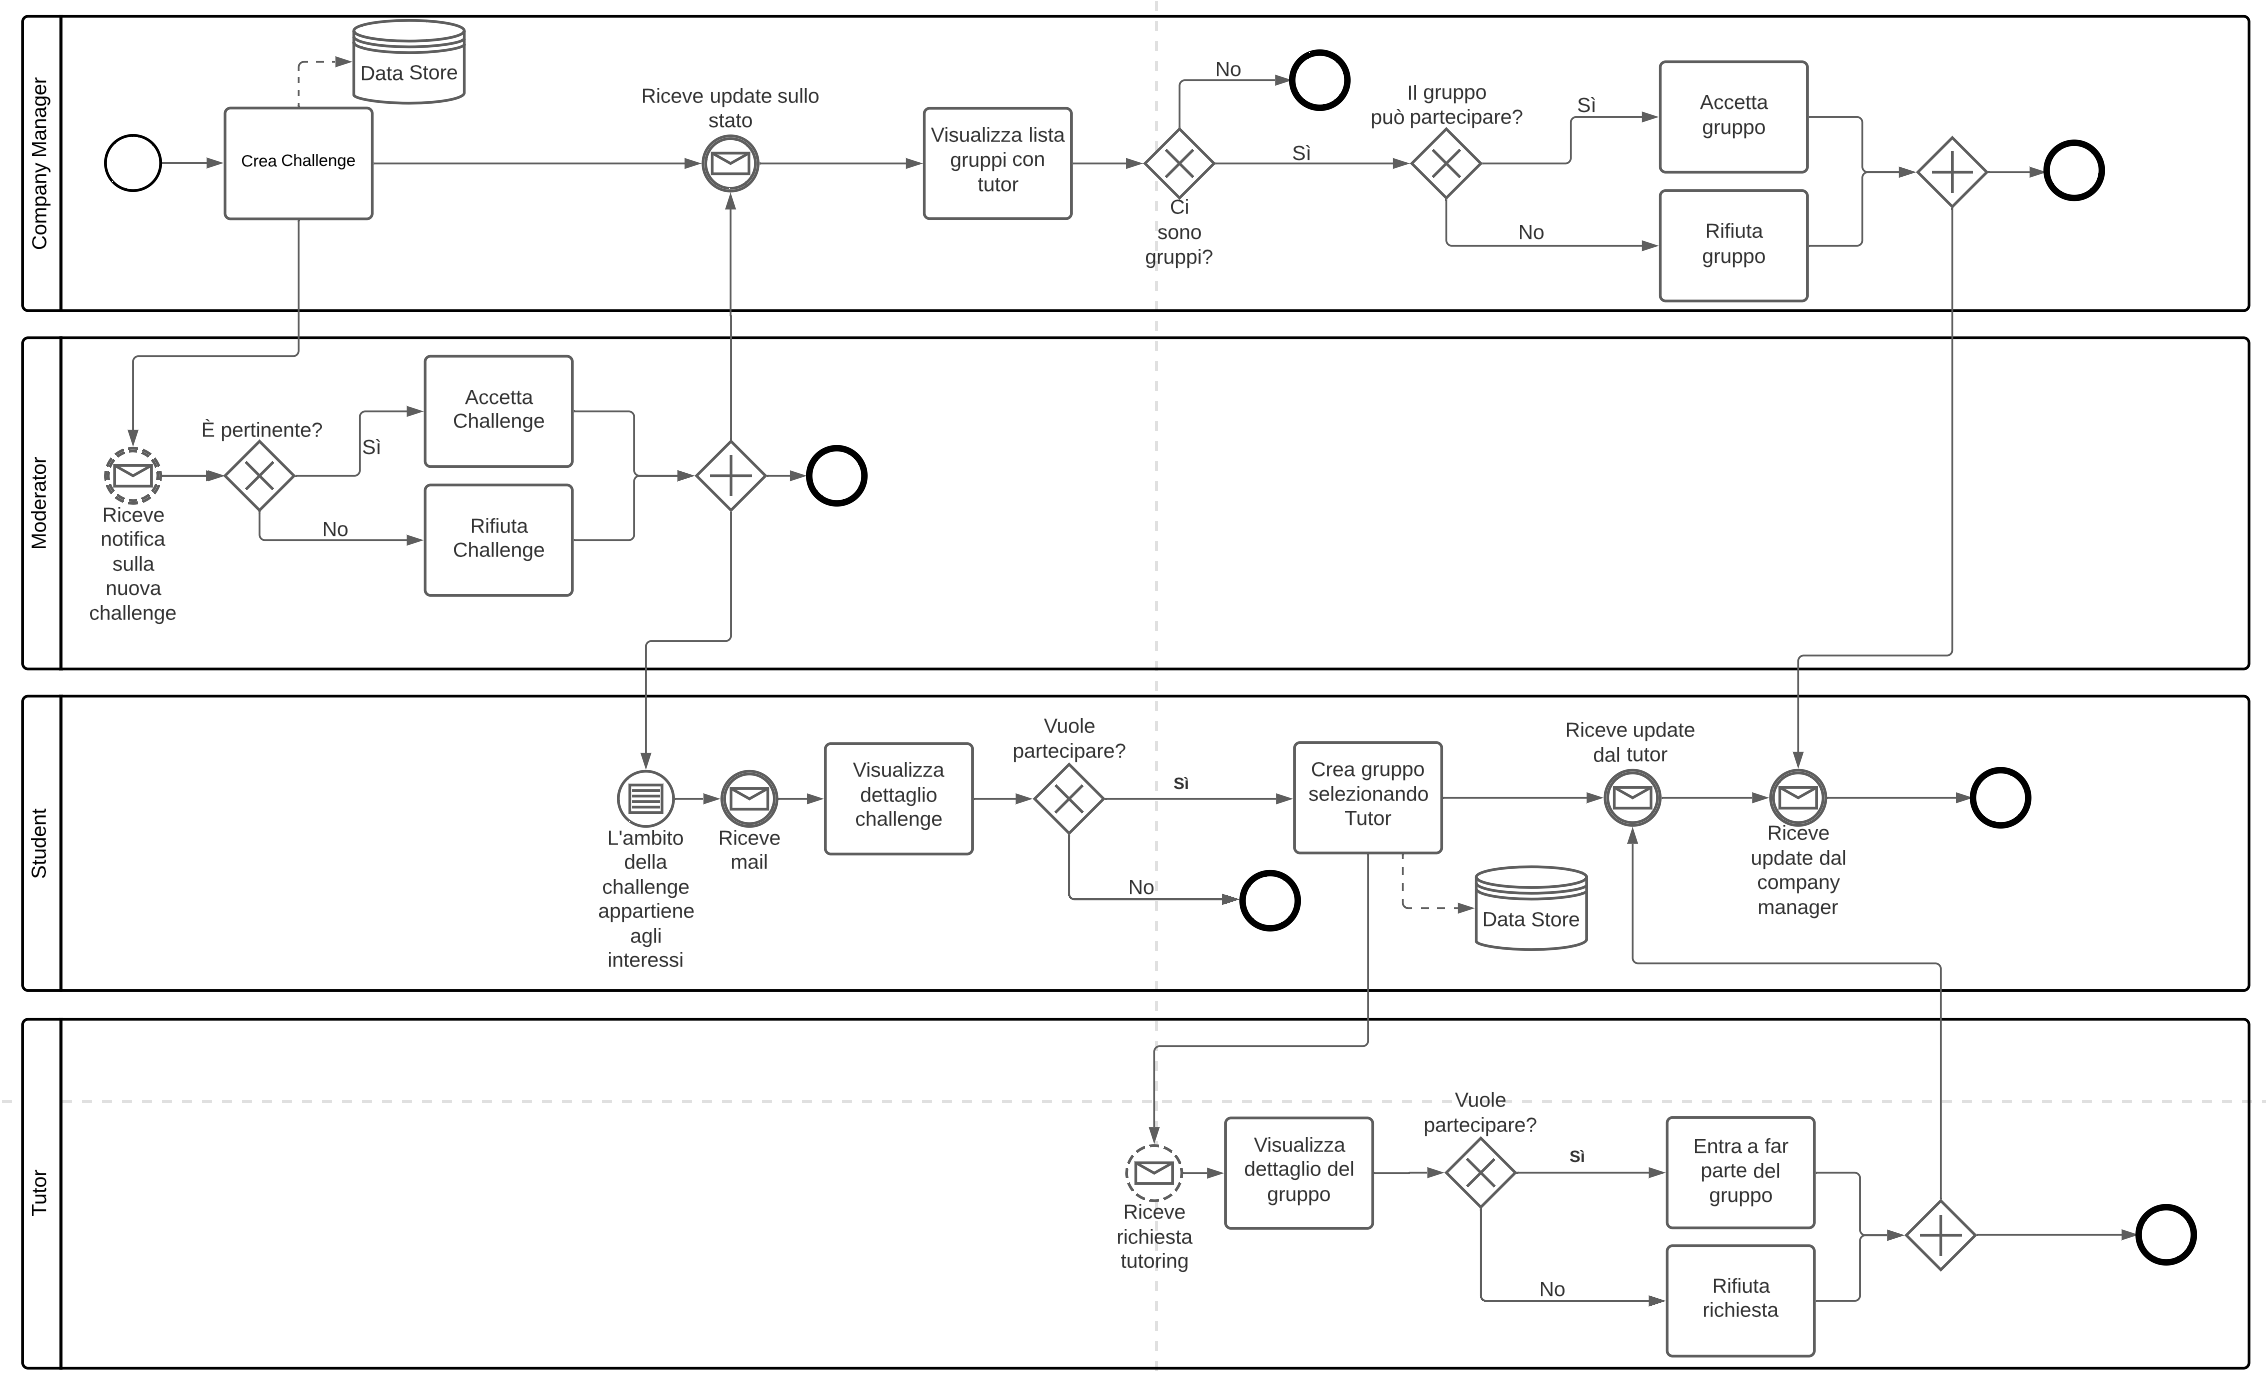
\includegraphics[width=0.95\textwidth]{images/BPMN_Challenge.png}
    \caption{BPMN della creazione di una Challenge}
    \label{fig:BPMN_Challenge}
\end{figure}

\clearpage

      

      \chapter{Conclusioni e sviluppi futuri}
\label{cha:conclusioni}
In questo capitolo vengono presentate le conclusioni ed i possibili sviluppi futuri dell'applicativo.

\section{Conclusioni}
Sono state presentate le varie fasi dello sviluppo dell'applicativo DISI Challenge, un progetto che rende possibile ridurre la distanza tra la realtà dell'industria con quella universitaria, permettendo alle aziende di formalizzare Challenges ed agli studenti di formare dei gruppi per accedervi, tutto in un'unica WebApp.

Prima dello sviluppo dell'applicativo, è stata svolta un'accurata analisi delle tecnologie utilizzate in DISI Industry, per permettere di avere un'applicazione che lavorasse in sintonia con essa, in modo da poter avere un'esperienza utente unica, senza dover imparare ad utilizzare due applicativi diversi.

Per quanto concerne gli obbiettivi definiti, essi sono stati raggiunti in quanto l'applicazione permette le seguenti operazioni da parte dei vari attori:
\begin{itemize}
    \item Company Manager : creazione e gestione delle Challenges, oltre al fornire dei feedback sulla qualità del lavoro svolto dagli studenti.
    \item Studenti : partecipazione alle Challenges proposte dalle varie aziende, formando dei gruppi e gestendoli, oltre alla possibilità di creare dei feedback per le Challenges alle quali si è partecipati.
\end{itemize}

Oltre a questi attori, i principali all'interno dell'applicativo, sono stati definiti degli attori di supporto, tra i quali Moderatori e Tutor, figure che permettono di avere un controllo maggiore all'interno dell'applicativo.


\section{Validazione}
Ad ogni funzionalità aggiunta si sono svolti degli Unit Tests, ossia dei test volti al verificare che tale funzionalità sia implementata correttamente. Inoltre è stato necessario verificare che tutte le nuove funzionalità implementate non andassero a modificare il comportamento delle funzionalità già presenti, per questo motivo sono stati svolti anche degli Integration Tests.

Per quanto concerne la validazione dell'applicativo e per poter ottenere dei feedback ulteriori a quelli già ottenuti, questo progetto verrà presentato all'azienda \textbf{Hub Innovazione Trentino} \cite{HiT}. Tale azienda è stata scelta proprio per le sue caratteristiche, in quanto essa congiunge il mondo accademico con quello dell'industria permettendo di introdurre innovazione in quest'ultimo, dunque ricevere un feedback da un possibile futuro utilizzatore è sicuramente un'ottima occasione per poter migliorare l'applicativo.


\section{Sviluppi Futuri}
L'applicazione ha visto un ingrandimento durante lo sviluppo, ad esempio con l'aggiunta del concetto di \textbf{Reputazione} \ref{sec:valutazioni}, non presente inizialmente. Per permettere di sviluppare tutti i requisiti cercando di mantenere il miglior standard qualitativo, sono state omesse alcune funzionalità ritenute secondarie.

Valutando la soluzione nel complesso, è possibile ottimizzare alcune query effettuate con il database per permettere di avere un'applicazione più performante. Un altra componente che può essere migliorata è il front-end, in quanto non essendo questo progetto solamente adibito a ciò ma essendo un progetto di ingegneria del software, è stato dato più peso alla parte di back-end, lasciando la parte di front-end più basilare e volta alla dimostrazione delle funzionalità richieste più che al lato estetico, comunque gradevole data l'estensione dallo stile dell'applicativo orginiale.


La principale funzionalità che potrebbe essere implementata è la parte di comunicazione tra studente ed azienda mediante una Chat all'interno dell'applicazione. Inizialmente DISI Challenge non era pensata per tale scopo, solamente che dopo aver analizzato DISI Industry ed aver notato la presenza di una forma di comunicazione già presente, è stata aggiunta questa funzionalità, non implementata in quanto secondaria nei confronti del funzionamento dell'applicativo come definito in fase iniziale, ossia di portale per la pubblicazione di Challenges e la loro duale funzionalità di iscrizione ad esse. Sarebbe dunque interessante vedere l'implementazione di un sistema di comunicazione all'interno dell'applicativo sfruttando le tecnologie già presenti in Industry, e ciò dovrebbe essere relativamente semplice data la particolare attenzione posta per rendere DISI Challenge un modulo che lavora in sintonia con DISI Industry.


      
      
    \endgroup


    % bibliografia in formato bibtex
    %
    % aggiunta del capitolo nell'indice
    \addcontentsline{toc}{chapter}{Bibliografia}
    % stile con ordinamento alfabetico in funzione degli autori
    \bibliographystyle{plain}
    \bibliography{biblio}
%%%%%%%%%%%%%%%%%%%%%%%%%%%%%%%%%%%%%%%%%%%%%%%%%%%%%%%%%%%%%%%%%%%%%%%%%%
%%%%%%%%%%%%%%%%%%%%%%%%%%%%%%%%%%%%%%%%%%%%%%%%%%%%%%%%%%%%%%%%%%%%%%%%%%
%% Nota
%%%%%%%%%%%%%%%%%%%%%%%%%%%%%%%%%%%%%%%%%%%%%%%%%%%%%%%%%%%%%%%%%%%%%%%%%%
%% Nella bibliografia devono essere riportati tutte le fonti consultate 
%% per lo svolgimento della tesi. La bibliografia deve essere redatta 
%% in ordine alfabetico sul cognome del primo autore. 
%% 
%% La forma della citazione bibliografica va inserita secondo la fonte utilizzata:
%% 
%% LIBRI
%% Cognome e iniziale del nome autore/autori, la data di edizione, titolo, casa editrice, eventuale numero dell’edizione. 
%% 
%% ARTICOLI DI RIVISTA
%% Cognome e iniziale del nome autore/autori, titolo articolo, titolo rivista, volume, numero, numero di pagine.
%% 
%% ARTICOLI DI CONFERENZA
%% Cognome e iniziale del nome autore/autori (anno), titolo articolo, titolo conferenza, luogo della conferenza (città e paese), date della conferenza, numero di pagine. 
%% 
%% SITOGRAFIA
%% La sitografia contiene un elenco di indirizzi Web consultati e disposti in ordine alfabetico. 
%% E’ necessario:
%%   Copiare la URL (l’indirizzo web) specifica della pagina consultata
%%   Se disponibile, indicare il cognome e nome dell’autore, il titolo ed eventuale sottotitolo del testo
%%   Se disponibile, inserire la data di ultima consultazione della risorsa (gg/mm/aaaa).
%%%%%%%%%%%%%%%%%%%%%%%%%%%%%%%%%%%%%%%%%%%%%%%%%%%%%%%%%%%%%%%%%%%%%%%%%%
%%%%%%%%%%%%%%%%%%%%%%%%%%%%%%%%%%%%%%%%%%%%%%%%%%%%%%%%%%%%%%%%%%%%%%%%%%
    

    \titleformat{\chapter}
        {\normalfont\Huge\bfseries}{Allegato \thechapter}{1em}{}
    % sezione Allegati - opzionale
    \appendix
\end{document}
